\documentclass[10pt,a4paper,fullpage]{article}

\usepackage[utf8]{inputenc}
\usepackage[T1]{fontenc}
\usepackage{amsmath}
\usepackage{amsfonts}
\usepackage{amssymb}
\usepackage{graphicx}
\usepackage{geometry}
\usepackage{array}
\usepackage{multirow}
\usepackage{caption}
\usepackage{booktabs}
\usepackage{titling}
\usepackage{float}

\geometry{a4paper, margin=1in}
\pagenumbering{gobble} 

\newcolumntype{C}[1]{>{\centering\let\newline\\\arraybackslash\hspace{0pt}}m{#1}}

\begin{document}

\title{Pattern Recognition - Exercise 2d (CNN \& MLP)}
\author{}
\predate{}
\postdate{}
\date{\vspace{-5ex}}
\maketitle


\textbf{Implementation details and Testing details}
\begin{itemize}
	\item See Report of Exercise 2b (MLP)
	\item See Report of Exercise 2c (CNN)
\end{itemize}

\textbf{Results for CNN permutated}
\begin{itemize}
	\item Number of epochs: 10
	\item Initial learning rate: 0.1
	\item Accuracy: 97.71\%
\end{itemize}

\vspace{-0.5cm}
\begin{center}
	\begin{tabular}{ r | c | c | c | c }
		\hline
		\multicolumn{1}{c|}{} & \multicolumn{2}{c|}{\textbf{Accuracy}} & \multicolumn{2}{c}{\textbf{Loss}}\\
		\hline
		\textbf{Epoch} & Train Dataset & Test Dataset & Train Dataset & Test Dataset\\
		\hline
		1 & 92.60\% & 92.70\% & 0.2568 & 0.2495 \\
		2 & 95.41\% & 95.20\% & 0.1604 & 0.1613 \\
		3 & 96.24\% & 95.85\% & 0.1336 & 0.1391 \\
		4 & 96.49\% & 96.11\% & 0.1190 & 0.1368 \\
		5 & 97.50\% & 96.61\% & 0.0914 & 0.1114 \\
		6 & 97.91\% & 96.69\% & 0.0844 & 0.1078 \\
		7 & 98.07\% & 97.15\% & 0.0773 & 0.0999 \\
		8 & 98.36\% & 97.18\% & 0.0644 & 0.0930 \\
		9 & 98.38\% & 97.15\% & 0.0583 & 0.0914 \\
		10 & 98.76\% & 97.34\% & 0.0505 & 0.0855 \\
		11 & 98.68\% & 97.20\% & 0.0519 & 0.0897 \\
		12 & 98.87\% & 97.38\% & 0.0471 & 0.0849 \\
		13 & 98.95\% & 97.51\% & 0.0411 & 0.0807 \\
		14 & 99.09\% & 97.60\% & 0.0386 & 0.0792 \\
		15 & 99.17\% & 97.56\% & 0.0357 & 0.0786 \\
		16 & 99.20\% & 97.57\% & 0.0352 & 0.0798 \\
		17 & 99.28\% & 97.65\% & 0.0333 & 0.0788 \\
		18 & 99.36\% & 97.64\% & 0.0303 & 0.0767 \\
		19 & 99.35\% & 97.66\% & 0.0307 & 0.0782 \\
		20 & 99.40\% & 97.71\% & 0.0283 & 0.0753 \\
		\hline
	\end{tabular}
\end{center}

% From https://timodenk.com/blog/exporting-matplotlib-plots-to-latex/
\begin{figure}[H]
	\begin{center}
		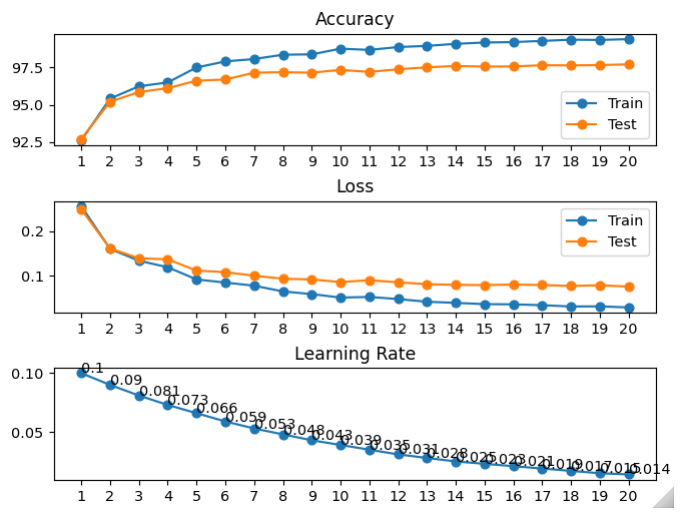
\includegraphics[scale=1]{cnn_model_plot_permutated.png}
	\end{center}
\end{figure}


\textbf{Comparision between CNN with normal dataset and CNN with permutated dataset}
\begin{itemize}
	\item The accuracy is slighly lower with the permutated MNIST dataset (98.60\% vs 97.71\%)
	\item The loss is slighly lower with the permutated MNIST dataset
	\item We clearly see that it is not a problem that the dataset given is permutated for the classification with the CNN 
\end{itemize}


\end{document}